155. Подпишем все отрезки на картинке с учётом того, что правый верхний прямоугольник является квадратом.
\begin{center}
\begin{figure}[ht!]
\center{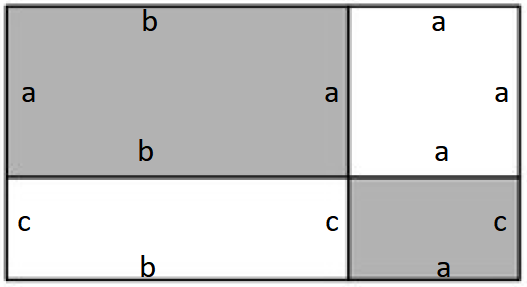
\includegraphics[scale=0.35]{37s.png}}
\end{figure}
\end{center}
Тогда $(a+b)\cdot2=34,\ a+b=17$см, $(a+c)\cdot2=22,\ a+c=11$см. Периметр всего прямоугольника равен $2\cdot(b+a+a+c)=2\cdot(17+11)=56$см. Его площадь равна $(b+a)(a+c)=17\cdot11=187\text{см}^2.$\newpage\noindent
